%Images of the complete circuits and PCBs
\subsection{Schematics}
Below is a presentation of the central schematics for the circuitry. In all cases where a power pin is used, a decoupling capacitor of 100nF is used. The schematics are presented in separate parts since the whole project is too large to get a good image of the complete system.
\begin{figure} [H]
\begin{center}
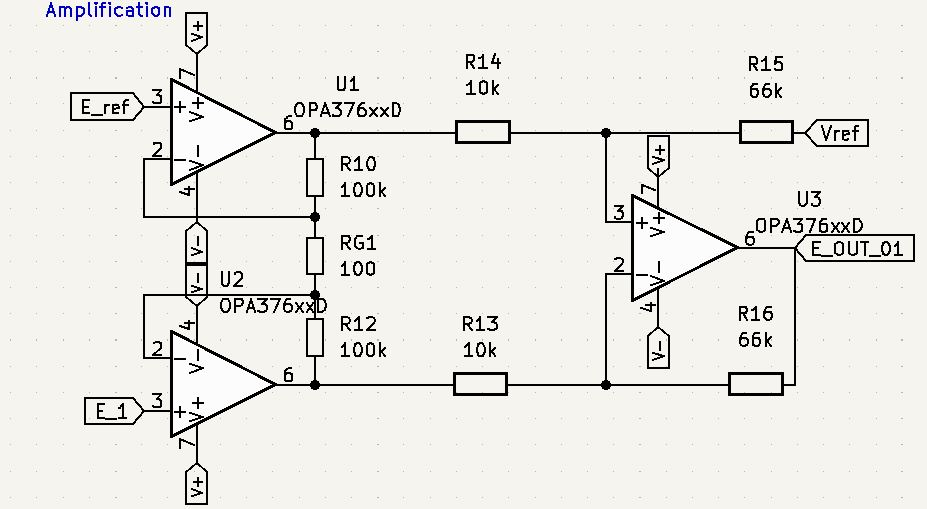
\includegraphics[scale=0.5]{images/Amplifiern.jpg}
   \caption{Instrumentation amplifier used to amplify the electrode signal and to suppress common mode noise}
    \label{fig:amplifier}
\end{center}
\end{figure}

\begin{figure} [H]
\begin{center}
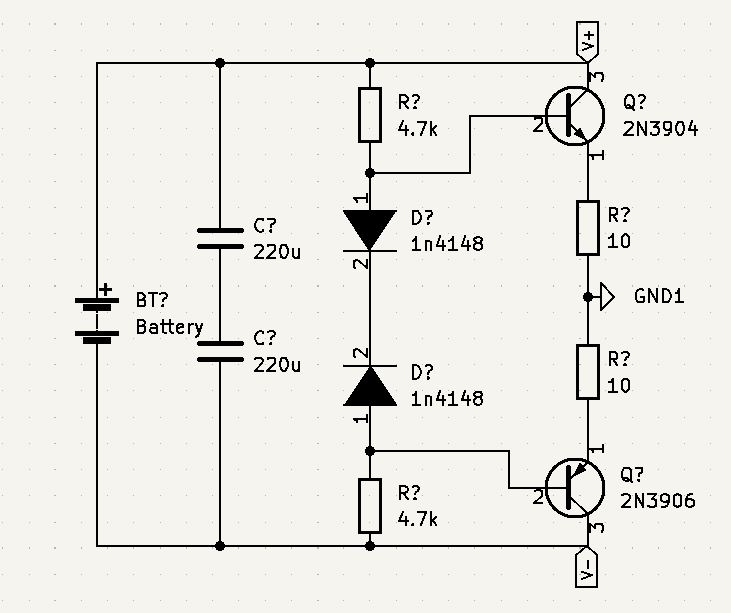
\includegraphics[scale=0.5]{images/Railsplitter.jpg}
   \caption{Rail splitter circuit designed after Sijosae Discreet Rail Splitter design \cite{railsplit}}
    \label{fig:railsplit}
\end{center}
\end{figure}

\begin{figure} [H]
\begin{center}
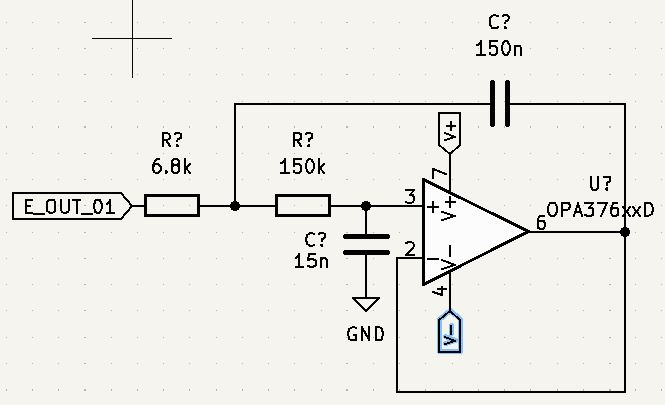
\includegraphics[scale=0.65]{images/Antialiasing.jpg}
   \caption{Second order Sallen-Key lowpass Butterworth filter used as anti aliasing filter}
    \label{fig:LPaliasfilter}
\end{center}
\end{figure}

\begin{figure} [H]
\begin{center}
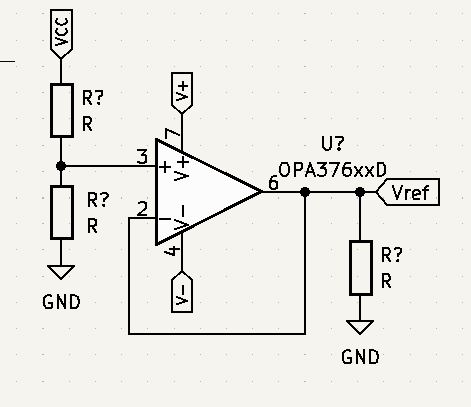
\includegraphics[scale=0.8]{images/Voltagebuffer.jpg}
   \caption{Voltage buffer used to get a stable $V_ref$ amplitude}
    \label{fig:Vbuff}
\end{center}
\end{figure}

\begin{figure} [H]
\begin{center}
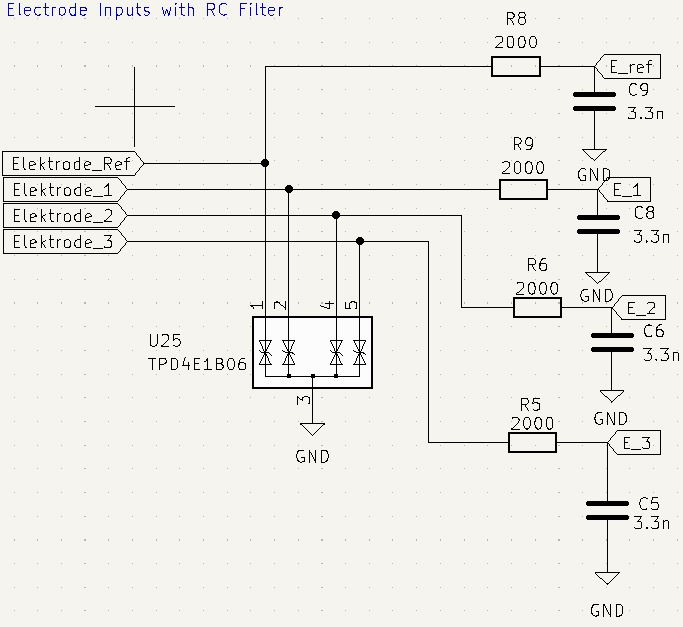
\includegraphics[scale=0.60]{images/Inputcirc.jpg}
   \caption{ESD protection and RC filter used on the electrode input}
    \label{fig:Elecinput}
\end{center}
\end{figure}

\begin{figure} [H]
\begin{center}
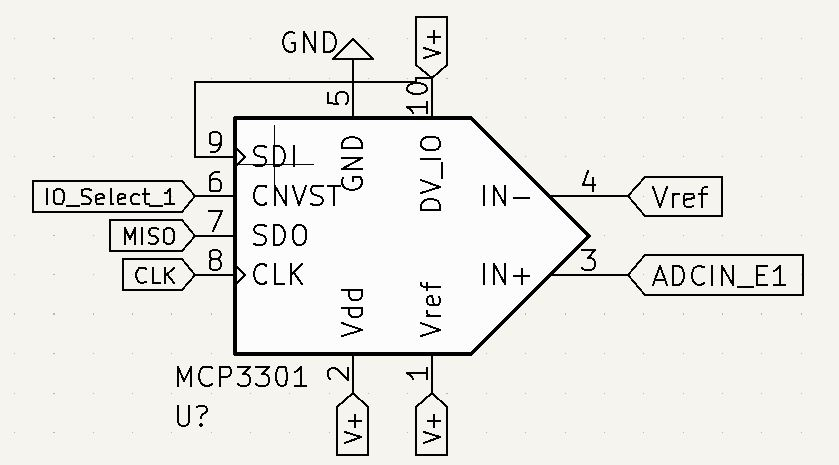
\includegraphics[scale=0.40]{images/ADC_CS_select.jpg}
   \caption{One of the possible ADC configurations using the CS line to select what chip is addressing the SPI line}
    \label{fig:ADC_CS}
\end{center}
\end{figure}
%Could maybe be removed hard to see anything useful
\begin{figure} [H]
\begin{center}
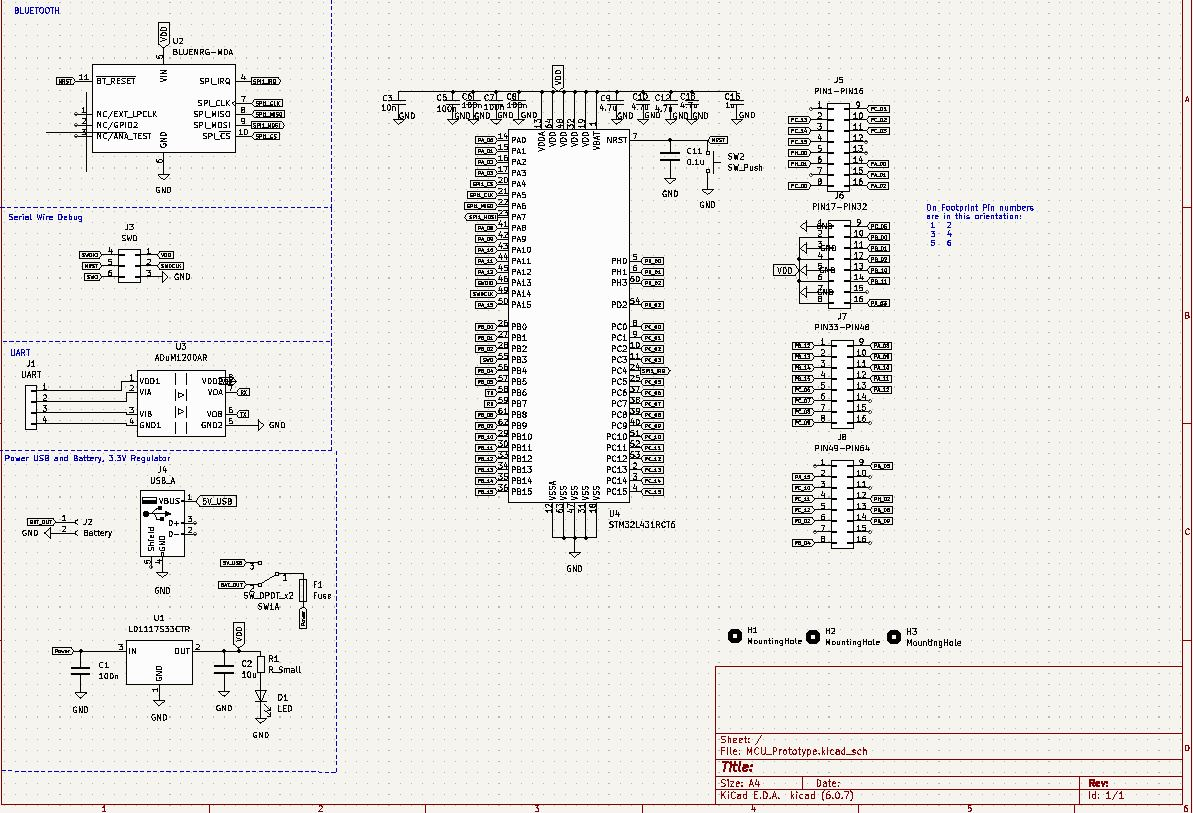
\includegraphics[scale=0.60,angle=-90]{images/FullcircMCU.jpg}
   \caption{The full circuit for the data processing PCB}
    \label{fig:MCUcirc}
\end{center}
\end{figure}

\begin{figure} [H]
\begin{center}
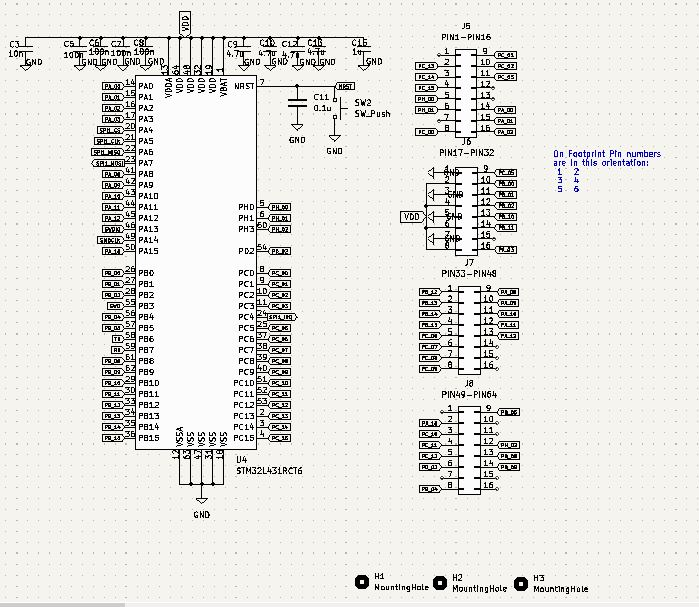
\includegraphics[scale=0.65]{images/MCU.jpg}
   \caption{The MCU configuration with proper decoupling}
    \label{fig:MCU}
\end{center}
\end{figure}

\begin{figure} [H]
\begin{center}
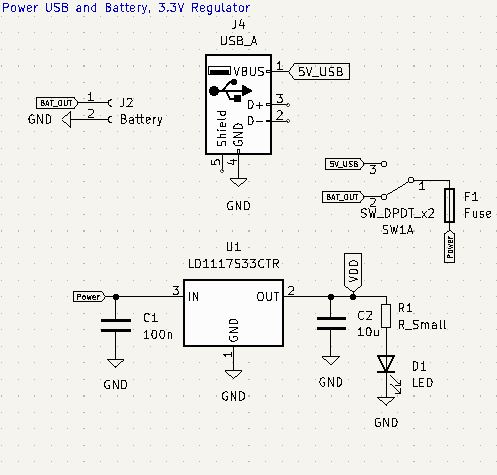
\includegraphics[scale=0.7]{images/Powercirc.jpg}
   \caption{Power circuit for the MCU board with a switch to choose between USB or battery power and a fuse to protect the board from malfunctions.}
    \label{fig:MCUpower}
\end{center}
\end{figure}

\begin{figure} [H]
\begin{center}
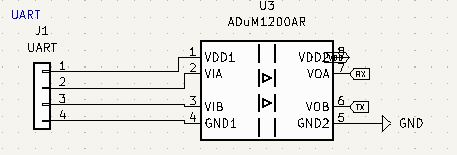
\includegraphics[scale=0.8]{images/UART.jpg}
   \caption{UART configuration with digital isolator}
    \label{fig:MCUuart}
\end{center}
\end{figure}

\begin{figure} [H]
\begin{center}
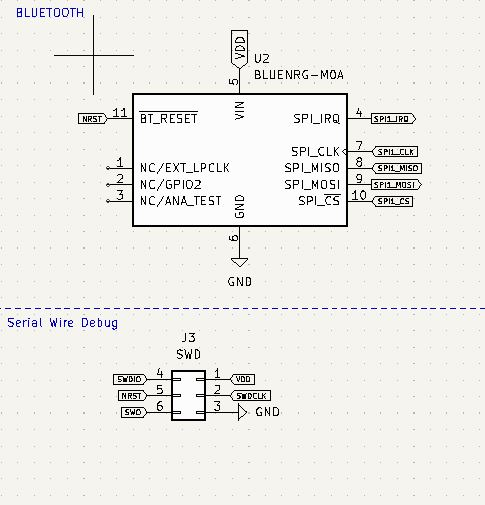
\includegraphics[scale=0.7]{images/BLE_SWD.jpg}
   \caption{Bluetooth configuration and SWD programming pins}
    \label{fig:MCUBLE}
\end{center}
\end{figure}
\subsection{PCBs}
\begin{figure} [H]
\begin{center}
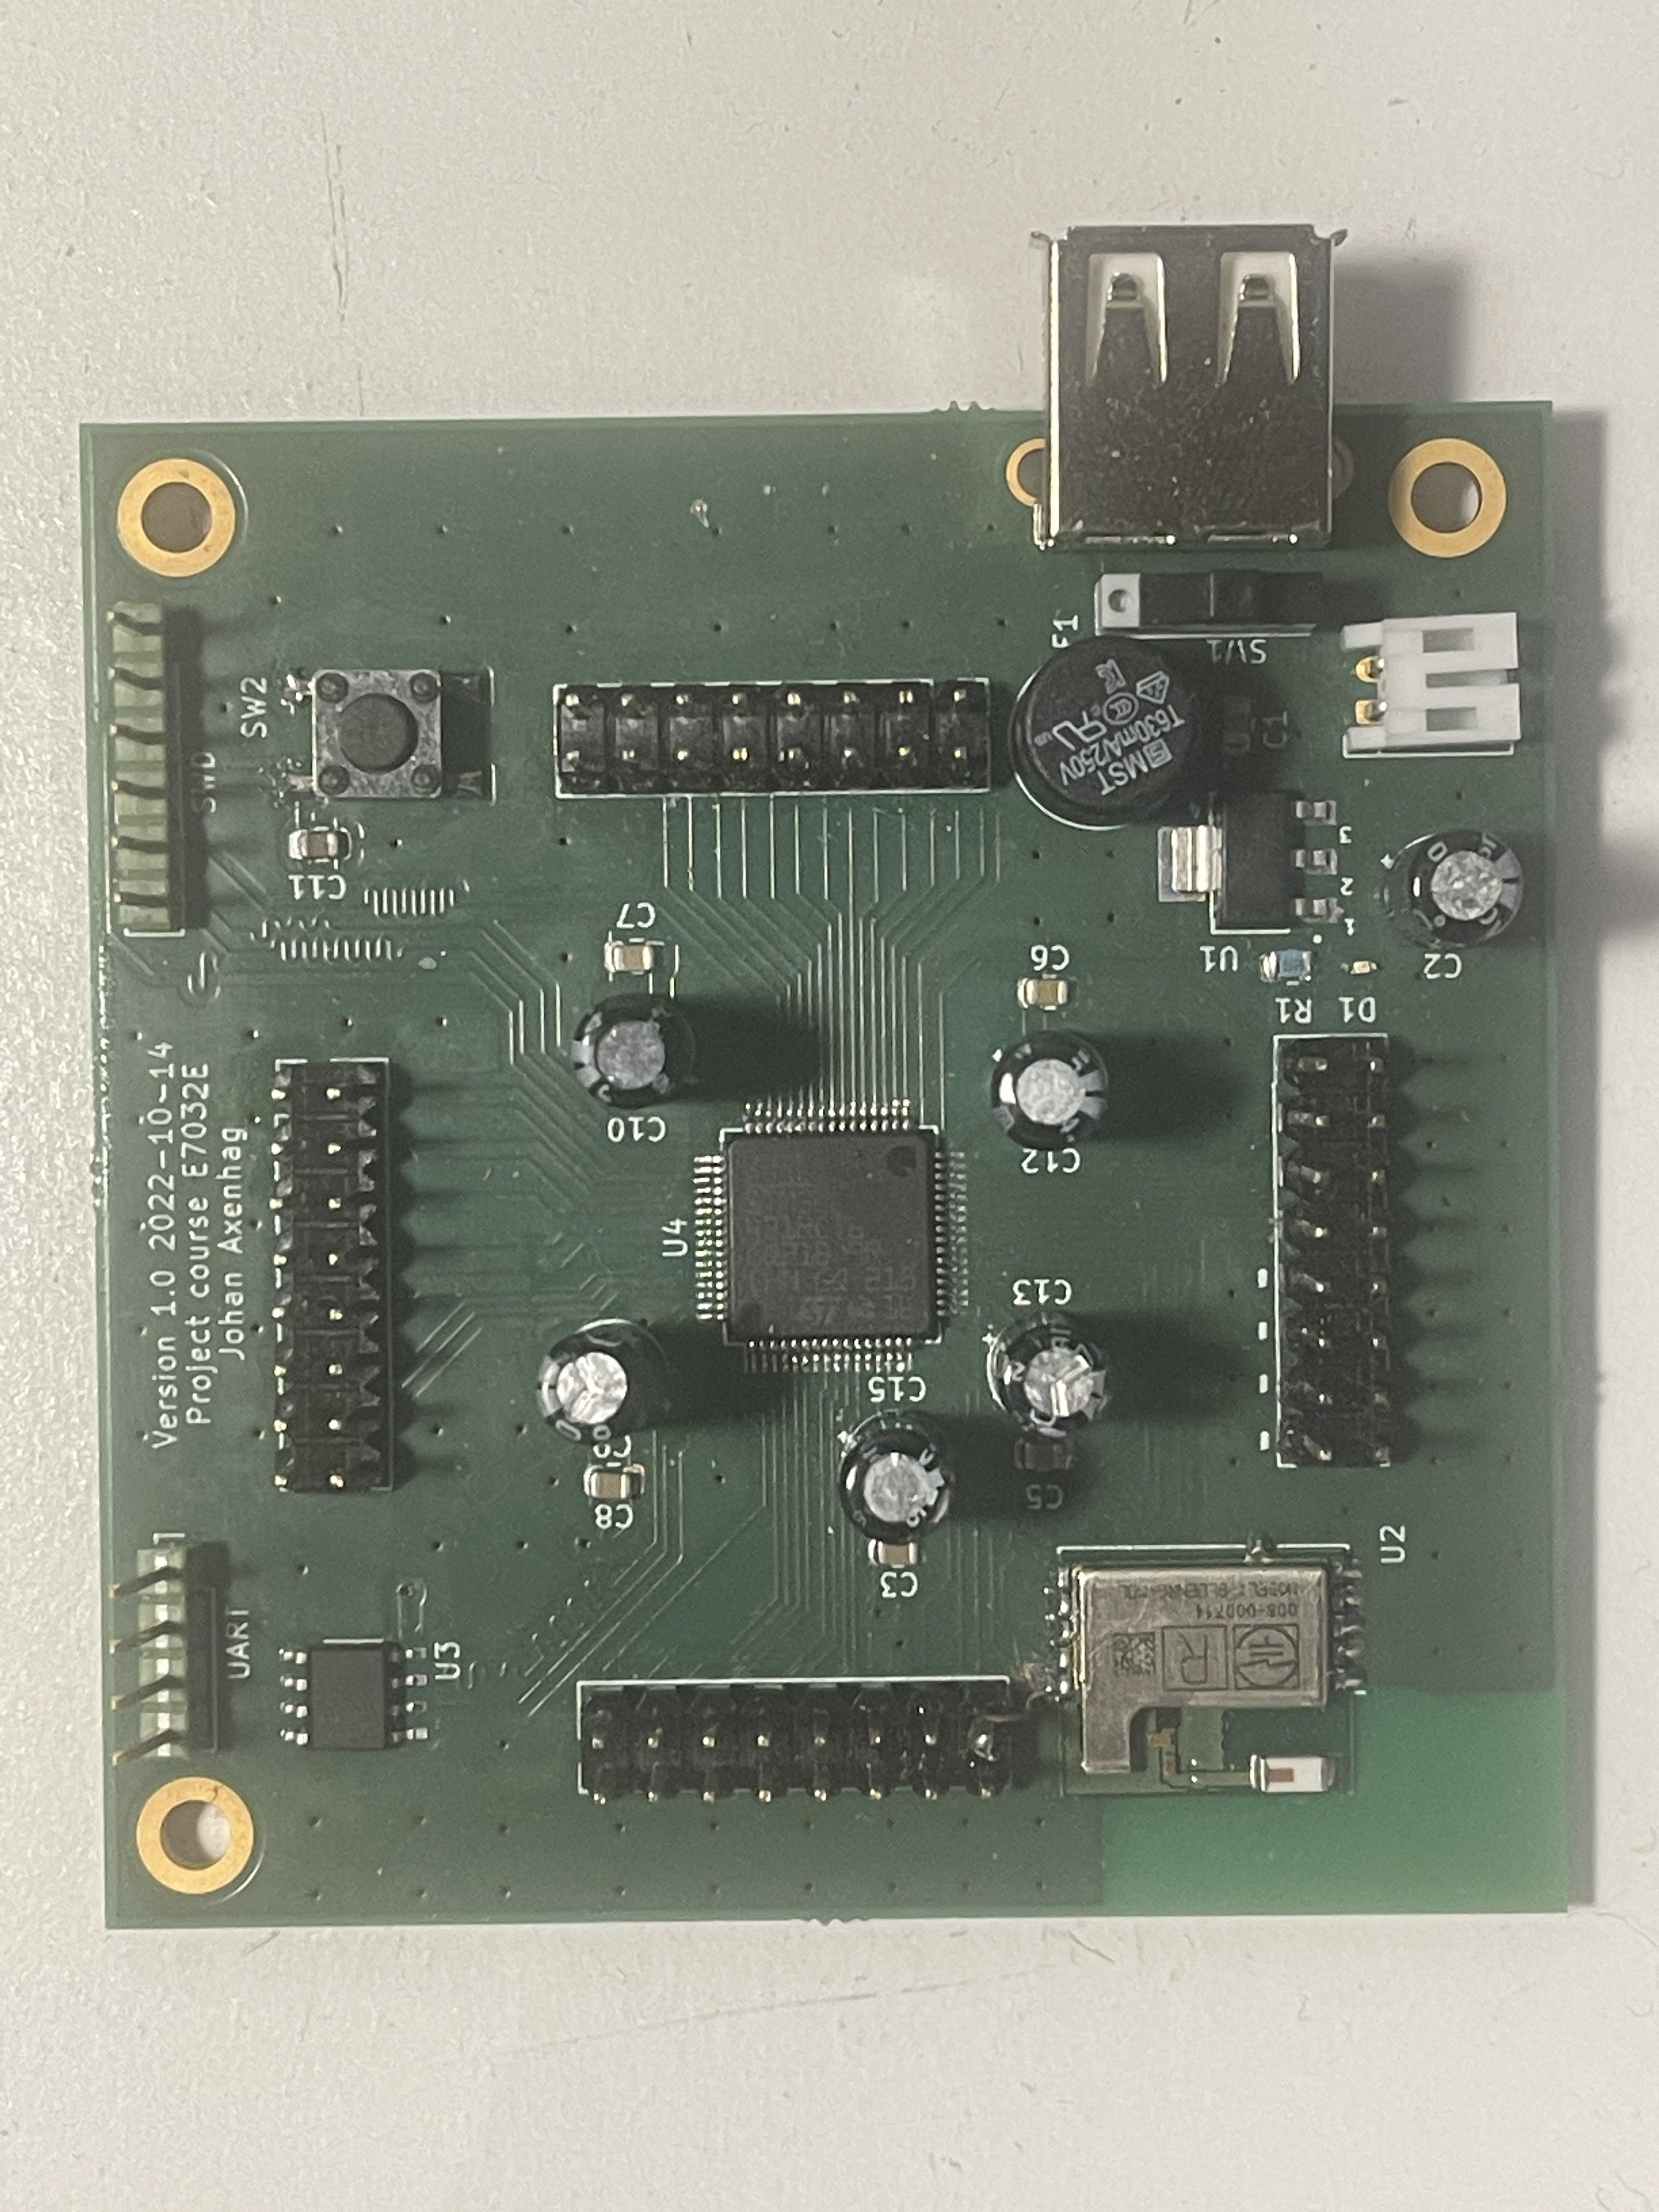
\includegraphics[width=\textwidth]{images/pcb.jpg}
   \caption{The main PCB containing the MCU and Bluetooth module}
    \label{fig:PCBData}
\end{center}
\end{figure}